\documentclass{article}
\usepackage[english]{babel}
\usepackage[utf8]{inputenc}
\usepackage[T1]{fontenc}
\usepackage{hyperref}
\usepackage[margin=0.5in]{geometry}
\usepackage{xspace}
%\usepackage{siunitx}
\usepackage{xcolor}
\usepackage{amsmath}
\usepackage{graphicx}
\usepackage{palatino}
\usepackage{microtype}

\newcommand{\sir}{\textsc{sir}\xspace}
\newcommand{\gspn}{\textsc{gspn}\xspace}

\title{Demographic, Stochastic SIR}
\author{Drew}

\begin{document}
\maketitle

\section{Introduction}
This document is about a little \sir simulation along the lines of the
time-dependent infection rate example from Wearing and others\cite{Wearing2012}.
We'll use the Semi-Markov library\cite{SemiMarkov2014} to do the simulation.

\section{ODE Model}
The model, as given in Wearing, is an \sir with birth and death.
Using $N=S+I+R$, $\mu$ as a death rate, $\gamma$ as a recovery rate,
and $\beta I/N$ as a freqency-dependent infection rate,
\begin{eqnarray}
  \frac{dS}{dt}&=& B - \frac{\beta I}{N}S-\mu S \\
  \frac{dI}{dt}&=& \frac{\beta I}{N}S-\gamma I-\mu I \\
  \frac{dR}{dt}&=& \gamma I - \mu R.
\end{eqnarray}
The crude birth rate, $B$, fixes asymptotic population size by breaking
scaling invariance, which you can see by adding the equations,
\begin{equation}
  \frac{dN}{dt}=B-\mu N.
\end{equation}
At long times and for fixed $\beta$,
\begin{eqnarray}
  N & = & B/\mu \\
  S & = & \frac{(\mu+\gamma)B}{\beta \mu} \\
  I & = & \frac{(\beta-\mu-\gamma)B}{\beta(\mu+\gamma)} \\
  R & = & \gamma I/\mu
\end{eqnarray}
The model seems well-behaved. We are interested in adding a seasonal
dependency to this model, so $\beta=\beta_0(1+\beta_1 \cos(2\pi (t-t_i))).$
Time is measured in years, here. The values used in the example
are \\
\begin{tabular}{ll}
B & 1/70 per year \\
$\beta$ & 400 per year \\
$\mu$ & 1/70 per year \\
$\gamma$ & 365/14 per year.
\end{tabular}
Note that $N=1$ with the choice of $B/\mu$.

\section{Stochastic Model}
For background on stochastic \sir, see Allen's chapter\cite{Allen:2008ma}.
Every transition in the stochastic model is exponential, which makes for
a simple system. There are three places, $S$, $I$, and $R$, with a transition
for each term of the differential equation. The \gspn is shown in Fig.~\ref{fig:sirgspn}.
\begin{figure}
\centerline{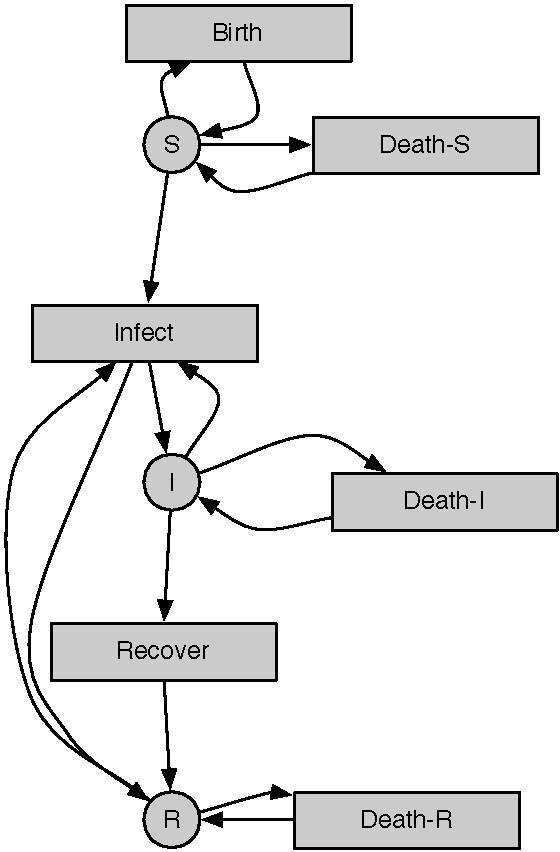
\includegraphics[scale=0.35]{sirexpgspn}}
\caption{The \gspn for the stochastic model. Note that the infection
transition includes inputs from all of $S$, $I$, and $R$ because it depends
on the total $N$ individuals.\label{fig:sirgspn}}
\end{figure}
Working from the figure, we list our transitions. \\
\begin{tabular}{ll}
  \hline
  Transition & Hazard Rate \\
  \hline
  birth & $B$ \\
  death-s & $\mu S$ \\
  death-i & $\mu I$ \\
  death-r & $\mu R$ \\
  infect & $\beta SI/(S+I+R)$ \\
  recover & $\gamma I$ \\
  \hline
\end{tabular}

The only complication is that the hazard rate will be seasonal,
\begin{equation}
  \beta(t)=\beta_0(1+\beta_1 \cos(2\pi (t-t_i))),
\end{equation}
where $t_i$ is an offset into the year and $\beta_1<1$. It is likely there will be enough
events per year that we can safely approximate this piecewise, but let's start
with the exact distribution because we can.
We can write this as
\begin{equation}
  \beta(t)=\beta_0(1+\beta_1 [\cos(2\pi t) \cos(2\pi t_i)+\sin(2\pi t) \sin(2\pi t_i)]).
\end{equation}
This hazard depends on the absolute system time but does not depend on
when an individual entered the susceptible state. We construct the
distribution for this transition, from the hazard rate, as
\begin{equation}
  F(t,t_0)=1-e^{-\int_{t_0}^t\beta_0(1+\beta_1 \cos(2\pi (s-t_i)))ds},
\end{equation}
which we will need to invert, $U=F(t,t_0)$, in order to sample.
Looking just at the integral,
\begin{equation}
  \int_{t_0}^t\beta_0(1+\beta_1 \cos(2\pi (s-t_i)))=\beta_0\left((t-t_0)+\frac{\beta_1}{2\pi}\sin(2\pi (t-t_i))-\frac{\beta_1}{2\pi}\sin(2\pi (t_0-t_i))\right)
\end{equation}
If we define $t_0'=t_0+\frac{\beta_1}{2\pi}\sin(2\pi (t_0-t_i)),$ then we
have to solve
\begin{equation}
  -\ln(1-U)/\beta_0+t_0'=t+\frac{\beta_1}{2\pi}\sin(2\pi (t-t_i)).
\end{equation}

% s(a-b)=sa cb - ca sb
% s(t-i)-s(o-i)=st ci - ct si -(so ci- co si)
% st ci - ct si - so ci + co si
% (st-so) ci - (ct-co) si

% s(t-o)=st co - ct so
% c(t-o)=ct co - st so

% mult by co
% st co ci - ct co si - so co ci + co co si

% add 

\bibliography{freqsir}
\bibliographystyle{plain}
\end{document}


